\documentclass[../informe.tex]{subfiles}
\begin{document}
As it can be seen on the figure \ref{cloud-service-architecture} the cloud service is divided by Subscriber, Producer, Consumer, DatabaseController and Queues.


\begin{figure}[!htbp]
    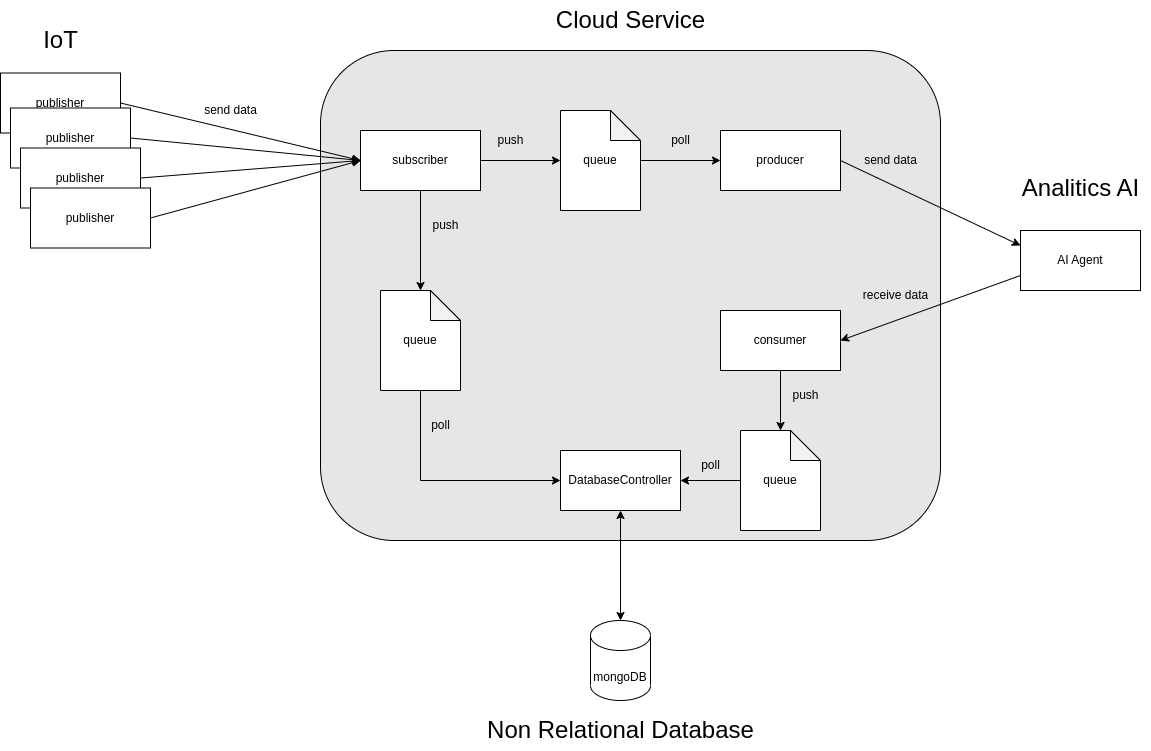
\includegraphics[scale=0.25]{cloud-service-architecture.png}
    \centering
    \caption{Cloud Service Architecture}
    \label{cloud-service-architecture}
\end{figure}

\newpage

\subsection{Subscriber}
This class defines an Subscriber thread that listens for incoming messages on a specified MQTT topic from a specified broker. When a message is received, it is deserialized and added to two queues, one for Kafka and one for a database. The Subscriber implements the MqttCallback interface to handle the various MQTT events. \\

It's worth noting that the run() method of the Subscriber class is calling itself if a connection is lost or an error occurs in order to try to reconnect to the specified broker. \\

\subsection{Producer}
This class defines a Kafka Producer thread that sends messages to a Kafka broker. It uses a PasiveWaitQueue to retrieve messages from a queue and sends them to the Kafka broker using a KafkaProducer. \\

The KafkaProducer is created using a set of properties that specify the configuration for the producer, such as the address of the Kafka broker and the serializers to use for the keys (StringSerializer) and values (TemperatureSerializer, which is a custom serializer) of the messages. \\

The run() method of the DataProducer thread continuously polls the PasiveWaitQueue for new messages and sends them to the Kafka broker. The message is a Temperature object, which is wrapped in a ProducerRecord and then sent to the Kafka broker using the send method of the KafkaProducer. \\


\subsection{Consumer}
This class defines a Kafka Consumer thread that consumes messages from a Kafka topic. It user a PasiveWaitQueue to send the messages received from the Kafka Broker to the KafkaDatabase controller. \\

The run() method is overridden to provide the behavior of the thread. It has a loop that polls the Kafka consumer for messages with a timeout of 100 milliseconds. For each message received, it pushes the value of the message (a TemperaturePrediction object) onto the PasiveWaitQueue object and prints some information about the message to the console. \\

The Kafka consumer is subscribed to the "analytics\_results" topic, so it will receive all messages published to that topic. The consumer is configured to start reading from the earliest record in the stream, and to use a custom deserializer for the values of the messages (TemperaturePredictionDeserializer). The group.id property is set to "predictions-results", which identifies the consumer group that this consumer belongs to. \\

\subsection{Database Controller}
This class defines a DatabaseController thread that starts two threads, one for the Kafka temperature predictions database controller, and one for the MQTT temperature data database controller. Both use the same InfluxDB client in order to store the data to the same database. \\

The token used to connect to the database is fix since it is specified like this on the docker-compose.yaml of the database. \\

\subsubsection{Kafka Database Controller}
This class defines the Kafka database controlled thread mentioned before. It continuously polls the PasiveWaitQueue given by the Database Controller for a TemperaturePrediction object, and then saves it to the database using the InfluxDBClient and its writeMeasurement method. \\

\subsubsection{MQTT Database Controller}
This class does the same as the Kafka Database Controller, but storing temperatures from the MQTT broker

\subsection{PasiveWaitQueue}
This is a thread-safe queue implementation that uses a ConcurrentLinkedQueue as the underlying data structure to store the elements. \\ 

There are two public methods (push and poll) and two private methods (isEmpty and waitData). The push method adds an element to the queue and then sends a notification to all waiting threads to wake up and check the queue for new data. The poll method waits for data to be available in the queue if it is empty, and then returns and removes the first element in the queue. The isEmpty method checks if the queue is empty. The waitData makes the execution wait to be notified. \\


One thing to note is that the waitData method calls wait on the queue object itself, which means that any thread that calls wait or notifyAll on the queue must hold the lock on the queue object. This is because the wait and notifyAll methods can only be called from within a synchronized block. \\

This implementation enables the usage of while(true) to poll data from the queue without doing an active wait. \\

\end{document}

